\documentclass[1p]{elsarticle_modified}
%\bibliographystyle{elsarticle-num}

%\usepackage[colorlinks]{hyperref}
%\usepackage{abbrmath_seonhwa} %\Abb, \Ascr, \Acal ,\Abf, \Afrak
\usepackage{amsfonts}
\usepackage{amssymb}
\usepackage{amsmath}
\usepackage{amsthm}
\usepackage{scalefnt}
\usepackage{amsbsy}
\usepackage{kotex}
\usepackage{caption}
\usepackage{subfig}
\usepackage{color}
\usepackage{graphicx}
\usepackage{xcolor} %% white, black, red, green, blue, cyan, magenta, yellow
\usepackage{float}
\usepackage{setspace}
\usepackage{hyperref}

\usepackage{tikz}
\usetikzlibrary{arrows}

\usepackage{multirow}
\usepackage{array} % fixed length table
\usepackage{hhline}

%%%%%%%%%%%%%%%%%%%%%
\makeatletter
\renewcommand*\env@matrix[1][\arraystretch]{%
	\edef\arraystretch{#1}%
	\hskip -\arraycolsep
	\let\@ifnextchar\new@ifnextchar
	\array{*\c@MaxMatrixCols c}}
\makeatother %https://tex.stackexchange.com/questions/14071/how-can-i-increase-the-line-spacing-in-a-matrix
%%%%%%%%%%%%%%%

\usepackage[normalem]{ulem}

\newcommand{\msout}[1]{\ifmmode\text{\sout{\ensuremath{#1}}}\else\sout{#1}\fi}
%SOURCE: \msout is \stkout macro in https://tex.stackexchange.com/questions/20609/strikeout-in-math-mode

\newcommand{\cancel}[1]{
	\ifmmode
	{\color{red}\msout{#1}}
	\else
	{\color{red}\sout{#1}}
	\fi
}

\newcommand{\add}[1]{
	{\color{blue}\uwave{#1}}
}

\newcommand{\replace}[2]{
	\ifmmode
	{\color{red}\msout{#1}}{\color{blue}\uwave{#2}}
	\else
	{\color{red}\sout{#1}}{\color{blue}\uwave{#2}}
	\fi
}

\newcommand{\Sol}{\mathcal{S}} %segment
\newcommand{\D}{D} %diagram
\newcommand{\A}{\mathcal{A}} %arc


%%%%%%%%%%%%%%%%%%%%%%%%%%%%%5 test

\def\sl{\operatorname{\textup{SL}}(2,\Cbb)}
\def\psl{\operatorname{\textup{PSL}}(2,\Cbb)}
\def\quan{\mkern 1mu \triangleright \mkern 1mu}

\theoremstyle{definition}
\newtheorem{thm}{Theorem}[section]
\newtheorem{prop}[thm]{Proposition}
\newtheorem{lem}[thm]{Lemma}
\newtheorem{ques}[thm]{Question}
\newtheorem{cor}[thm]{Corollary}
\newtheorem{defn}[thm]{Definition}
\newtheorem{exam}[thm]{Example}
\newtheorem{rmk}[thm]{Remark}
\newtheorem{alg}[thm]{Algorithm}

\newcommand{\I}{\sqrt{-1}}
\begin{document}

%\begin{frontmatter}
%
%\title{Boundary parabolic representations of knots up to 8 crossings}
%
%%% Group authors per affiliation:
%\author{Yunhi Cho} 
%\address{Department of Mathematics, University of Seoul, Seoul, Korea}
%\ead{yhcho@uos.ac.kr}
%
%
%\author{Seonhwa Kim} %\fnref{s_kim}}
%\address{Center for Geometry and Physics, Institute for Basic Science, Pohang, 37673, Korea}
%\ead{ryeona17@ibs.re.kr}
%
%\author{Hyuk Kim}
%\address{Department of Mathematical Sciences, Seoul National University, Seoul 08826, Korea}
%\ead{hyukkim@snu.ac.kr}
%
%\author{Seokbeom Yoon}
%\address{Department of Mathematical Sciences, Seoul National University, Seoul, 08826,  Korea}
%\ead{sbyoon15@snu.ac.kr}
%
%\begin{abstract}
%We find all boundary parabolic representation of knots up to 8 crossings.
%
%\end{abstract}
%\begin{keyword}
%    \MSC[2010] 57M25 
%\end{keyword}
%
%\end{frontmatter}

%\linenumbers
%\tableofcontents
%
\newcommand\colored[1]{\textcolor{white}{\rule[-0.35ex]{0.8em}{1.4ex}}\kern-0.8em\color{red} #1}%
%\newcommand\colored[1]{\textcolor{white}{ #1}\kern-2.17ex	\textcolor{white}{ #1}\kern-1.81ex	\textcolor{white}{ #1}\kern-2.15ex\color{red}#1	}

{\Large $\underline{12a_{0999}~(K12a_{0999})}$}

\setlength{\tabcolsep}{10pt}
\renewcommand{\arraystretch}{1.6}
\vspace{1cm}\begin{tabular}{m{100pt}>{\centering\arraybackslash}m{274pt}}
\multirow{5}{120pt}{
	\centering
	\includegraphics[width=112pt]{../../../GIT/diagram.site/Diagrams/png/1800_12a_0999.png}\\
\ \ \ A knot diagram\footnotemark}&
\allowdisplaybreaks
\textbf{Linearized knot diagam} \\
\cline{2-2}
 &
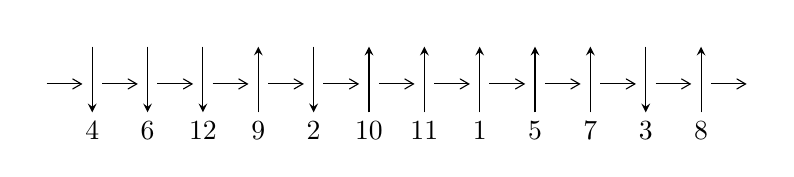
\begin{tikzpicture}[x=20pt, y=17pt]
	% nodes
	\node (C0) at (0, 0) {};
	\node (C1) at (1, 0) {};
	\node (C1U) at (1, +1) {};
	\node (C1D) at (1, -1) {4};

	\node (C2) at (2, 0) {};
	\node (C2U) at (2, +1) {};
	\node (C2D) at (2, -1) {6};

	\node (C3) at (3, 0) {};
	\node (C3U) at (3, +1) {};
	\node (C3D) at (3, -1) {12};

	\node (C4) at (4, 0) {};
	\node (C4U) at (4, +1) {};
	\node (C4D) at (4, -1) {9};

	\node (C5) at (5, 0) {};
	\node (C5U) at (5, +1) {};
	\node (C5D) at (5, -1) {2};

	\node (C6) at (6, 0) {};
	\node (C6U) at (6, +1) {};
	\node (C6D) at (6, -1) {10};

	\node (C7) at (7, 0) {};
	\node (C7U) at (7, +1) {};
	\node (C7D) at (7, -1) {11};

	\node (C8) at (8, 0) {};
	\node (C8U) at (8, +1) {};
	\node (C8D) at (8, -1) {1};

	\node (C9) at (9, 0) {};
	\node (C9U) at (9, +1) {};
	\node (C9D) at (9, -1) {5};

	\node (C10) at (10, 0) {};
	\node (C10U) at (10, +1) {};
	\node (C10D) at (10, -1) {7};

	\node (C11) at (11, 0) {};
	\node (C11U) at (11, +1) {};
	\node (C11D) at (11, -1) {3};

	\node (C12) at (12, 0) {};
	\node (C12U) at (12, +1) {};
	\node (C12D) at (12, -1) {8};
	\node (C13) at (13, 0) {};

	% arrows
	\draw[->,>={angle 60}]
	(C0) edge (C1) (C1) edge (C2) (C2) edge (C3) (C3) edge (C4) (C4) edge (C5) (C5) edge (C6) (C6) edge (C7) (C7) edge (C8) (C8) edge (C9) (C9) edge (C10) (C10) edge (C11) (C11) edge (C12) (C12) edge (C13) ;	\draw[->,>=stealth]
	(C1U) edge (C1D) (C2U) edge (C2D) (C3U) edge (C3D) (C4D) edge (C4U) (C5U) edge (C5D) (C6D) edge (C6U) (C7D) edge (C7U) (C8D) edge (C8U) (C9D) edge (C9U) (C10D) edge (C10U) (C11U) edge (C11D) (C12D) edge (C12U) ;
	\end{tikzpicture} \\
\hhline{~~} \\& 
\textbf{Solving Sequence} \\ \cline{2-2} 
 &
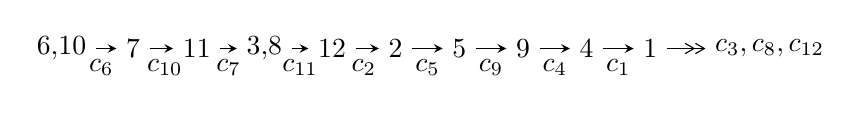
\begin{tikzpicture}[x=23pt, y=7pt]
	% node
	\node (A0) at (-1/8, 0) {6,10};
	\node (A1) at (1, 0) {7};
	\node (A2) at (2, 0) {11};
	\node (A3) at (49/16, 0) {3,8};
	\node (A4) at (33/8, 0) {12};
	\node (A5) at (41/8, 0) {2};
	\node (A6) at (49/8, 0) {5};
	\node (A7) at (57/8, 0) {9};
	\node (A8) at (65/8, 0) {4};
	\node (A9) at (73/8, 0) {1};
	\node (C1) at (1/2, -1) {$c_{6}$};
	\node (C2) at (3/2, -1) {$c_{10}$};
	\node (C3) at (5/2, -1) {$c_{7}$};
	\node (C4) at (29/8, -1) {$c_{11}$};
	\node (C5) at (37/8, -1) {$c_{2}$};
	\node (C6) at (45/8, -1) {$c_{5}$};
	\node (C7) at (53/8, -1) {$c_{9}$};
	\node (C8) at (61/8, -1) {$c_{4}$};
	\node (C9) at (69/8, -1) {$c_{1}$};
	\node (A10) at (11, 0) {$c_{3},c_{8},c_{12}$};

	% edge
	\draw[->,>=stealth]	
	(A0) edge (A1) (A1) edge (A2) (A2) edge (A3) (A3) edge (A4) (A4) edge (A5) (A5) edge (A6) (A6) edge (A7) (A7) edge (A8) (A8) edge (A9) ;
	\draw[->>,>={angle 60}]	
	(A9) edge (A10);
\end{tikzpicture} \\ 

\end{tabular} \\

\footnotetext{
The image of knot diagram is generated by the software ``\textbf{Draw programme}" developed by Andrew Bartholomew(\url{http://www.layer8.co.uk/maths/draw/index.htm\#Running-draw}), where we modified some parts for our purpose(\url{https://github.com/CATsTAILs/LinksPainter}).
}\phantom \\ \newline 
\centering \textbf{Ideals for irreducible components\footnotemark of $X_{\text{par}}$} 
 
\begin{align*}
I^u_{1}&=\langle 
826872493 u^{24}+41514578887 u^{23}+\cdots+26691174904 b+267919895192,\\
\phantom{I^u_{1}}&\phantom{= \langle  }75775316763 u^{24}-724263180731 u^{23}+\cdots+53382349808 a-515069062880,\\
\phantom{I^u_{1}}&\phantom{= \langle  }u^{25}-11 u^{24}+\cdots-80 u+16\rangle \\
I^u_{2}&=\langle 
-10 u^{35}-12 u^{34}+\cdots+8 b+68,\;-68 u^{35} a+508 u^{35}+\cdots-1145 a+7276,\;u^{36}+4 u^{35}+\cdots+16 u+1\rangle \\
I^u_{3}&=\langle 
-7 u^{10}+4 u^9+36 u^8-34 u^7-43 u^6+60 u^5+10 u^4-31 u^3-19 u^2+11 b+16 u+17,\\
\phantom{I^u_{3}}&\phantom{= \langle  }-8 u^{10}+25 u^9+38 u^8-163 u^7+31 u^6+298 u^5-262 u^4-136 u^3+269 u^2+11 a-32 u-78,\\
\phantom{I^u_{3}}&\phantom{= \langle  }u^{11}-2 u^{10}-5 u^9+14 u^8+u^7-27 u^6+18 u^5+15 u^4-20 u^3- u^2+6 u+1\rangle \\
\\
I^v_{1}&=\langle 
a,\;b+1,\;v+1\rangle \\
\end{align*}
\raggedright * 4 irreducible components of $\dim_{\mathbb{C}}=0$, with total 109 representations.\\
\footnotetext{All coefficients of polynomials are rational numbers. But the coefficients are sometimes approximated in decimal forms when there is not enough margin.}
\newpage
\renewcommand{\arraystretch}{1}
\centering \section*{I. $I^u_{1}= \langle 8.27\times10^{8} u^{24}+4.15\times10^{10} u^{23}+\cdots+2.67\times10^{10} b+2.68\times10^{11},\;7.58\times10^{10} u^{24}-7.24\times10^{11} u^{23}+\cdots+5.34\times10^{10} a-5.15\times10^{11},\;u^{25}-11 u^{24}+\cdots-80 u+16 \rangle$}
\flushleft \textbf{(i) Arc colorings}\\
\begin{tabular}{m{7pt} m{180pt} m{7pt} m{180pt} }
\flushright $a_{6}=$&$\begin{pmatrix}1\\0\end{pmatrix}$ \\
\flushright $a_{10}=$&$\begin{pmatrix}0\\u\end{pmatrix}$ \\
\flushright $a_{7}=$&$\begin{pmatrix}1\\- u^2\end{pmatrix}$ \\
\flushright $a_{11}=$&$\begin{pmatrix}u\\- u^3+u\end{pmatrix}$ \\
\flushright $a_{3}=$&$\begin{pmatrix}-1.41948 u^{24}+13.5675 u^{23}+\cdots-51.2819 u+9.64868\\-0.0309792 u^{24}-1.55537 u^{23}+\cdots+37.1258 u-10.0378\end{pmatrix}$ \\
\flushright $a_{8}=$&$\begin{pmatrix}- u^2+1\\u^4-2 u^2\end{pmatrix}$ \\
\flushright $a_{12}=$&$\begin{pmatrix}0.167582 u^{24}-3.50276 u^{23}+\cdots+58.5852 u-16.0667\\3.79748 u^{24}-34.4987 u^{23}+\cdots+133.770 u-29.2311\end{pmatrix}$ \\
\flushright $a_{2}=$&$\begin{pmatrix}-1.45046 u^{24}+12.0121 u^{23}+\cdots-14.1561 u-0.389094\\-0.0309792 u^{24}-1.55537 u^{23}+\cdots+37.1258 u-10.0378\end{pmatrix}$ \\
\flushright $a_{5}=$&$\begin{pmatrix}3.96506 u^{24}-38.0015 u^{23}+\cdots+190.355 u-44.2978\\3.79748 u^{24}-34.4987 u^{23}+\cdots+132.770 u-29.2311\end{pmatrix}$ \\
\flushright $a_{9}=$&$\begin{pmatrix}-1.73754 u^{24}+15.9703 u^{23}+\cdots-68.0866 u+14.9573\\0.976986 u^{24}-8.80582 u^{23}+\cdots+24.7513 u-4.30668\end{pmatrix}$ \\
\flushright $a_{4}=$&$\begin{pmatrix}6.50025 u^{24}-60.8358 u^{23}+\cdots+275.705 u-62.6895\\-2.16560 u^{24}+22.8582 u^{23}+\cdots-153.338 u+36.8239\end{pmatrix}$ \\
\flushright $a_{1}=$&$\begin{pmatrix}-4.43829 u^{24}+41.9516 u^{23}+\cdots-195.816 u+43.9195\\-1.35725 u^{24}+12.5528 u^{23}+\cdots-50.4134 u+10.8323\end{pmatrix}$\\&\end{tabular}
\flushleft \textbf{(ii) Obstruction class $= -1$}\\~\\
\flushleft \textbf{(iii) Cusp Shapes $= \frac{145412112683}{3336396863} u^{24}-\frac{1365948008373}{3336396863} u^{23}+\cdots+\frac{6268794612260}{3336396863} u-\frac{1430304974606}{3336396863}$}\\~\\
\newpage\renewcommand{\arraystretch}{1}
\flushleft \textbf{(iv) u-Polynomials at the component}\newline \\
\begin{tabular}{m{50pt}|m{274pt}}
Crossings & \hspace{64pt}u-Polynomials at each crossing \\
\hline $$\begin{aligned}c_{1}\end{aligned}$$&$\begin{aligned}
&u^{25}-22 u^{24}+\cdots+5120 u+512
\end{aligned}$\\
\hline $$\begin{aligned}c_{2},c_{3},c_{5}\\c_{11}\end{aligned}$$&$\begin{aligned}
&u^{25}- u^{24}+\cdots-4 u+1
\end{aligned}$\\
\hline $$\begin{aligned}c_{4},c_{8},c_{9}\\c_{12}\end{aligned}$$&$\begin{aligned}
&u^{25}-11 u^{23}+\cdots+u-1
\end{aligned}$\\
\hline $$\begin{aligned}c_{6},c_{7},c_{10}\end{aligned}$$&$\begin{aligned}
&u^{25}-11 u^{24}+\cdots-80 u+16
\end{aligned}$\\
\hline
\end{tabular}\\~\\
\newpage\renewcommand{\arraystretch}{1}
\flushleft \textbf{(v) Riley Polynomials at the component}\newline \\
\begin{tabular}{m{50pt}|m{274pt}}
Crossings & \hspace{64pt}Riley Polynomials at each crossing \\
\hline $$\begin{aligned}c_{1}\end{aligned}$$&$\begin{aligned}
&y^{25}-2 y^{24}+\cdots+76808192 y-262144
\end{aligned}$\\
\hline $$\begin{aligned}c_{2},c_{3},c_{5}\\c_{11}\end{aligned}$$&$\begin{aligned}
&y^{25}-15 y^{24}+\cdots+50 y-1
\end{aligned}$\\
\hline $$\begin{aligned}c_{4},c_{8},c_{9}\\c_{12}\end{aligned}$$&$\begin{aligned}
&y^{25}-22 y^{24}+\cdots+21 y-1
\end{aligned}$\\
\hline $$\begin{aligned}c_{6},c_{7},c_{10}\end{aligned}$$&$\begin{aligned}
&y^{25}-23 y^{24}+\cdots-1408 y-256
\end{aligned}$\\
\hline
\end{tabular}\\~\\
\newpage\flushleft \textbf{(vi) Complex Volumes and Cusp Shapes}
$$\begin{array}{c|c|c}  
\text{Solutions to }I^u_{1}& \I (\text{vol} + \sqrt{-1}CS) & \text{Cusp shape}\\
 \hline 
\begin{aligned}
u &= -1.00934\phantom{ +0.000000I} \\
a &= -0.805015\phantom{ +0.000000I} \\
b &= \phantom{-}1.63266\phantom{ +0.000000I}\end{aligned}
 & -7.20191\phantom{ +0.000000I} & \phantom{-}30.6470\phantom{ +0.000000I} \\ \hline\begin{aligned}
u &= \phantom{-}0.012976 + 1.033860 I \\
a &= \phantom{-}0.633148 - 0.106162 I \\
b &= \phantom{-}0.791764 + 0.522766 I\end{aligned}
 & \phantom{-}3.03037 - 1.54703 I & \phantom{-}6.68506 + 3.68219 I \\ \hline\begin{aligned}
u &= \phantom{-}0.012976 - 1.033860 I \\
a &= \phantom{-}0.633148 + 0.106162 I \\
b &= \phantom{-}0.791764 - 0.522766 I\end{aligned}
 & \phantom{-}3.03037 + 1.54703 I & \phantom{-}6.68506 - 3.68219 I \\ \hline\begin{aligned}
u &= -0.881775 + 0.323566 I \\
a &= -0.378664 + 0.249573 I \\
b &= \phantom{-}0.365509 - 0.726585 I\end{aligned}
 & \phantom{-}6.42854 - 2.68579 I & \phantom{-}9.83614 + 1.93428 I \\ \hline\begin{aligned}
u &= -0.881775 - 0.323566 I \\
a &= -0.378664 - 0.249573 I \\
b &= \phantom{-}0.365509 + 0.726585 I\end{aligned}
 & \phantom{-}6.42854 + 2.68579 I & \phantom{-}9.83614 - 1.93428 I \\ \hline\begin{aligned}
u &= -0.477303 + 0.717814 I \\
a &= \phantom{-}0.009597 - 0.906421 I \\
b &= \phantom{-}1.269930 + 0.185562 I\end{aligned}
 & -7.01624 - 2.33284 I & -5.90770 + 2.60194 I \\ \hline\begin{aligned}
u &= -0.477303 - 0.717814 I \\
a &= \phantom{-}0.009597 + 0.906421 I \\
b &= \phantom{-}1.269930 - 0.185562 I\end{aligned}
 & -7.01624 + 2.33284 I & -5.90770 - 2.60194 I \\ \hline\begin{aligned}
u &= -0.482722 + 1.037880 I \\
a &= -0.369971 + 0.530061 I \\
b &= -1.214990 - 0.563112 I\end{aligned}
 & \phantom{-}1.10842 - 12.71280 I & \phantom{-}2.59152 + 8.71606 I \\ \hline\begin{aligned}
u &= -0.482722 - 1.037880 I \\
a &= -0.369971 - 0.530061 I \\
b &= -1.214990 + 0.563112 I\end{aligned}
 & \phantom{-}1.10842 + 12.71280 I & \phantom{-}2.59152 - 8.71606 I \\ \hline\begin{aligned}
u &= \phantom{-}1.329560 + 0.203875 I \\
a &= \phantom{-}0.28740 - 1.62065 I \\
b &= -0.662175 + 0.545556 I\end{aligned}
 & \phantom{-}2.65006 + 2.55544 I & \phantom{-}3.11128 - 1.65198 I\\
 \hline 
 \end{array}$$\newpage$$\begin{array}{c|c|c}  
\text{Solutions to }I^u_{1}& \I (\text{vol} + \sqrt{-1}CS) & \text{Cusp shape}\\
 \hline 
\begin{aligned}
u &= \phantom{-}1.329560 - 0.203875 I \\
a &= \phantom{-}0.28740 + 1.62065 I \\
b &= -0.662175 - 0.545556 I\end{aligned}
 & \phantom{-}2.65006 - 2.55544 I & \phantom{-}3.11128 + 1.65198 I \\ \hline\begin{aligned}
u &= -0.98981 + 1.06101 I \\
a &= \phantom{-}0.181907 + 0.253452 I \\
b &= -0.954754 + 0.361220 I\end{aligned}
 & \phantom{-}2.30832 + 5.78881 I & \phantom{-}2.00000 - 7.25000 I \\ \hline\begin{aligned}
u &= -0.98981 - 1.06101 I \\
a &= \phantom{-}0.181907 - 0.253452 I \\
b &= -0.954754 - 0.361220 I\end{aligned}
 & \phantom{-}2.30832 - 5.78881 I & \phantom{-}2.00000 + 7.25000 I \\ \hline\begin{aligned}
u &= \phantom{-}0.516035\phantom{ +0.000000I} \\
a &= \phantom{-}0.631196\phantom{ +0.000000I} \\
b &= \phantom{-}0.157637\phantom{ +0.000000I}\end{aligned}
 & \phantom{-}0.767709\phantom{ +0.000000I} & \phantom{-}13.0610\phantom{ +0.000000I} \\ \hline\begin{aligned}
u &= \phantom{-}1.49267 + 0.27371 I \\
a &= -0.65793 + 1.31350 I \\
b &= \phantom{-}1.148310 - 0.509995 I\end{aligned}
 & -0.65901 + 5.99024 I & \phantom{-0.000000 } 0. - 4.38665 I \\ \hline\begin{aligned}
u &= \phantom{-}1.49267 - 0.27371 I \\
a &= -0.65793 - 1.31350 I \\
b &= \phantom{-}1.148310 + 0.509995 I\end{aligned}
 & -0.65901 - 5.99024 I & \phantom{-0.000000 -}0. + 4.38665 I \\ \hline\begin{aligned}
u &= \phantom{-}1.47479 + 0.50270 I \\
a &= \phantom{-}0.123556 + 1.187480 I \\
b &= \phantom{-}1.108500 - 0.652505 I\end{aligned}
 & \phantom{-}7.77371 + 7.32084 I & \phantom{-}7.72526 - 5.56309 I \\ \hline\begin{aligned}
u &= \phantom{-}1.47479 - 0.50270 I \\
a &= \phantom{-}0.123556 - 1.187480 I \\
b &= \phantom{-}1.108500 + 0.652505 I\end{aligned}
 & \phantom{-}7.77371 - 7.32084 I & \phantom{-}7.72526 + 5.56309 I \\ \hline\begin{aligned}
u &= \phantom{-}1.58061 + 0.03704 I \\
a &= -0.272956 - 1.225950 I \\
b &= \phantom{-}0.151992 + 1.145230 I\end{aligned}
 & \phantom{-}14.6920 + 3.8040 I & \phantom{-}11.54426 - 2.08774 I \\ \hline\begin{aligned}
u &= \phantom{-}1.58061 - 0.03704 I \\
a &= -0.272956 + 1.225950 I \\
b &= \phantom{-}0.151992 - 1.145230 I\end{aligned}
 & \phantom{-}14.6920 - 3.8040 I & \phantom{-}11.54426 + 2.08774 I\\
 \hline 
 \end{array}$$\newpage$$\begin{array}{c|c|c}  
\text{Solutions to }I^u_{1}& \I (\text{vol} + \sqrt{-1}CS) & \text{Cusp shape}\\
 \hline 
\begin{aligned}
u &= \phantom{-}1.54138 + 0.37767 I \\
a &= \phantom{-}0.30399 - 1.46629 I \\
b &= -1.36369 + 0.77531 I\end{aligned}
 & \phantom{-}7.5940 + 17.7952 I & \phantom{-}5.80164 - 8.80793 I \\ \hline\begin{aligned}
u &= \phantom{-}1.54138 - 0.37767 I \\
a &= \phantom{-}0.30399 + 1.46629 I \\
b &= -1.36369 - 0.77531 I\end{aligned}
 & \phantom{-}7.5940 - 17.7952 I & \phantom{-}5.80164 + 8.80793 I \\ \hline\begin{aligned}
u &= \phantom{-}0.123896 + 0.326612 I \\
a &= -1.67598 + 1.41797 I \\
b &= -0.709073 - 0.106576 I\end{aligned}
 & -1.292320 - 0.176707 I & -7.01154 + 0.09257 I \\ \hline\begin{aligned}
u &= \phantom{-}0.123896 - 0.326612 I \\
a &= -1.67598 - 1.41797 I \\
b &= -0.709073 + 0.106576 I\end{aligned}
 & -1.292320 + 0.176707 I & -7.01154 - 0.09257 I \\ \hline\begin{aligned}
u &= \phantom{-}2.04475\phantom{ +0.000000I} \\
a &= \phantom{-}0.305643\phantom{ +0.000000I} \\
b &= -0.652933\phantom{ +0.000000I}\end{aligned}
 & \phantom{-}13.8003\phantom{ +0.000000I} & \phantom{-0.000000 } 0\\
 \hline 
 \end{array}$$\newpage\newpage\renewcommand{\arraystretch}{1}
\centering \section*{II. $I^u_{2}= \langle -10 u^{35}-12 u^{34}+\cdots+8 b+68,\;-68 u^{35} a+508 u^{35}+\cdots-1145 a+7276,\;u^{36}+4 u^{35}+\cdots+16 u+1 \rangle$}
\flushleft \textbf{(i) Arc colorings}\\
\begin{tabular}{m{7pt} m{180pt} m{7pt} m{180pt} }
\flushright $a_{6}=$&$\begin{pmatrix}1\\0\end{pmatrix}$ \\
\flushright $a_{10}=$&$\begin{pmatrix}0\\u\end{pmatrix}$ \\
\flushright $a_{7}=$&$\begin{pmatrix}1\\- u^2\end{pmatrix}$ \\
\flushright $a_{11}=$&$\begin{pmatrix}u\\- u^3+u\end{pmatrix}$ \\
\flushright $a_{3}=$&$\begin{pmatrix}a\\\frac{5}{4} u^{35}+\frac{3}{2} u^{34}+\cdots+\frac{57}{8} u-\frac{17}{2}\end{pmatrix}$ \\
\flushright $a_{8}=$&$\begin{pmatrix}- u^2+1\\u^4-2 u^2\end{pmatrix}$ \\
\flushright $a_{12}=$&$\begin{pmatrix}-\frac{5}{4} u^{35} a-2 u^{35}+\cdots+\frac{17}{2} a-\frac{439}{8}\\\frac{27}{8} u^{35}+\frac{59}{8} u^{34}+\cdots+\frac{123}{4} u-\frac{53}{8}\end{pmatrix}$ \\
\flushright $a_{2}=$&$\begin{pmatrix}\frac{5}{4} u^{35}+\frac{3}{2} u^{34}+\cdots+a-\frac{17}{2}\\\frac{5}{4} u^{35}+\frac{3}{2} u^{34}+\cdots+\frac{57}{8} u-\frac{17}{2}\end{pmatrix}$ \\
\flushright $a_{5}=$&$\begin{pmatrix}2.37500 a u^{35}+6.62500 a u^{34}+\cdots+3.12500 a-23.5000\\\frac{47}{8} u^{35} a-2 u^{35}+\cdots+\frac{35}{8} a-\frac{635}{8}\end{pmatrix}$ \\
\flushright $a_{9}=$&$\begin{pmatrix}\frac{1}{2} u^{35} a-\frac{41}{8} u^{35}+\cdots+\frac{37}{4} a-\frac{385}{8}\\-\frac{9}{4} u^{35} a+\frac{63}{8} u^{35}+\cdots-\frac{5}{2} a+84\end{pmatrix}$ \\
\flushright $a_{4}=$&$\begin{pmatrix}-2 u^{35} a+\frac{67}{2} u^{35}+\cdots-\frac{627}{8} a+\frac{1065}{2}\\\frac{27}{8} u^{35} a+u^{35}+\cdots+\frac{11}{4} a-\frac{15}{4}\end{pmatrix}$ \\
\flushright $a_{1}=$&$\begin{pmatrix}-2 u^{35} a+u^{35}+\cdots+\frac{61}{8} a-\frac{495}{8}\\-\frac{31}{8} u^{35} a+3 u^{35}+\cdots-\frac{23}{8} a-\frac{55}{8}\end{pmatrix}$\\&\end{tabular}
\flushleft \textbf{(ii) Obstruction class $= -1$}\\~\\
\flushleft \textbf{(iii) Cusp Shapes $= 148 u^{35}+\frac{1111}{2} u^{34}+\cdots+1907 u+\frac{3931}{2}$}\\~\\
\newpage\renewcommand{\arraystretch}{1}
\flushleft \textbf{(iv) u-Polynomials at the component}\newline \\
\begin{tabular}{m{50pt}|m{274pt}}
Crossings & \hspace{64pt}u-Polynomials at each crossing \\
\hline $$\begin{aligned}c_{1}\end{aligned}$$&$\begin{aligned}
&(u^{36}+11 u^{35}+\cdots+12 u+1)^{2}
\end{aligned}$\\
\hline $$\begin{aligned}c_{2},c_{3},c_{5}\\c_{11}\end{aligned}$$&$\begin{aligned}
&u^{72}+5 u^{71}+\cdots+44 u+31
\end{aligned}$\\
\hline $$\begin{aligned}c_{4},c_{8},c_{9}\\c_{12}\end{aligned}$$&$\begin{aligned}
&u^{72}+15 u^{71}+\cdots+1022 u+149
\end{aligned}$\\
\hline $$\begin{aligned}c_{6},c_{7},c_{10}\end{aligned}$$&$\begin{aligned}
&(u^{36}+4 u^{35}+\cdots+16 u+1)^{2}
\end{aligned}$\\
\hline
\end{tabular}\\~\\
\newpage\renewcommand{\arraystretch}{1}
\flushleft \textbf{(v) Riley Polynomials at the component}\newline \\
\begin{tabular}{m{50pt}|m{274pt}}
Crossings & \hspace{64pt}Riley Polynomials at each crossing \\
\hline $$\begin{aligned}c_{1}\end{aligned}$$&$\begin{aligned}
&(y^{36}+9 y^{35}+\cdots-78 y+1)^{2}
\end{aligned}$\\
\hline $$\begin{aligned}c_{2},c_{3},c_{5}\\c_{11}\end{aligned}$$&$\begin{aligned}
&y^{72}-109 y^{71}+\cdots-5904 y+961
\end{aligned}$\\
\hline $$\begin{aligned}c_{4},c_{8},c_{9}\\c_{12}\end{aligned}$$&$\begin{aligned}
&y^{72}-125 y^{71}+\cdots+239896 y+22201
\end{aligned}$\\
\hline $$\begin{aligned}c_{6},c_{7},c_{10}\end{aligned}$$&$\begin{aligned}
&(y^{36}-36 y^{35}+\cdots-228 y+1)^{2}
\end{aligned}$\\
\hline
\end{tabular}\\~\\
\newpage\flushleft \textbf{(vi) Complex Volumes and Cusp Shapes}
$$\begin{array}{c|c|c}  
\text{Solutions to }I^u_{2}& \I (\text{vol} + \sqrt{-1}CS) & \text{Cusp shape}\\
 \hline 
\begin{aligned}
u &= \phantom{-}0.801734 + 0.696202 I \\
a &= \phantom{-}0.525131 - 0.532417 I \\
b &= -1.060570 - 0.298701 I\end{aligned}
 & -2.58334 - 1.89748 I & -1.79078 + 1.73365 I \\ \hline\begin{aligned}
u &= \phantom{-}0.801734 + 0.696202 I \\
a &= -0.146921 + 0.381228 I \\
b &= \phantom{-}1.240490 + 0.042488 I\end{aligned}
 & -2.58334 - 1.89748 I & -1.79078 + 1.73365 I \\ \hline\begin{aligned}
u &= \phantom{-}0.801734 - 0.696202 I \\
a &= \phantom{-}0.525131 + 0.532417 I \\
b &= -1.060570 + 0.298701 I\end{aligned}
 & -2.58334 + 1.89748 I & -1.79078 - 1.73365 I \\ \hline\begin{aligned}
u &= \phantom{-}0.801734 - 0.696202 I \\
a &= -0.146921 - 0.381228 I \\
b &= \phantom{-}1.240490 - 0.042488 I\end{aligned}
 & -2.58334 + 1.89748 I & -1.79078 - 1.73365 I \\ \hline\begin{aligned}
u &= \phantom{-}0.406976 + 0.842772 I \\
a &= \phantom{-}0.364285 + 0.941569 I \\
b &= \phantom{-}1.216290 - 0.277018 I\end{aligned}
 & -3.72449 + 7.15532 I & -1.32336 - 7.08750 I \\ \hline\begin{aligned}
u &= \phantom{-}0.406976 + 0.842772 I \\
a &= -0.346677 - 0.608804 I \\
b &= -1.251710 + 0.596442 I\end{aligned}
 & -3.72449 + 7.15532 I & -1.32336 - 7.08750 I \\ \hline\begin{aligned}
u &= \phantom{-}0.406976 - 0.842772 I \\
a &= \phantom{-}0.364285 - 0.941569 I \\
b &= \phantom{-}1.216290 + 0.277018 I\end{aligned}
 & -3.72449 - 7.15532 I & -1.32336 + 7.08750 I \\ \hline\begin{aligned}
u &= \phantom{-}0.406976 - 0.842772 I \\
a &= -0.346677 + 0.608804 I \\
b &= -1.251710 - 0.596442 I\end{aligned}
 & -3.72449 - 7.15532 I & -1.32336 + 7.08750 I \\ \hline\begin{aligned}
u &= -0.392598 + 1.003430 I \\
a &= -0.903413 - 0.103360 I \\
b &= -0.821320 - 0.340230 I\end{aligned}
 & \phantom{-}2.79209 + 2.82464 I & \phantom{-}5.35953 - 2.15606 I \\ \hline\begin{aligned}
u &= -0.392598 + 1.003430 I \\
a &= \phantom{-}0.442073 - 0.041027 I \\
b &= \phantom{-}0.867684 - 0.552611 I\end{aligned}
 & \phantom{-}2.79209 + 2.82464 I & \phantom{-}5.35953 - 2.15606 I\\
 \hline 
 \end{array}$$\newpage$$\begin{array}{c|c|c}  
\text{Solutions to }I^u_{2}& \I (\text{vol} + \sqrt{-1}CS) & \text{Cusp shape}\\
 \hline 
\begin{aligned}
u &= -0.392598 - 1.003430 I \\
a &= -0.903413 + 0.103360 I \\
b &= -0.821320 + 0.340230 I\end{aligned}
 & \phantom{-}2.79209 - 2.82464 I & \phantom{-}5.35953 + 2.15606 I \\ \hline\begin{aligned}
u &= -0.392598 - 1.003430 I \\
a &= \phantom{-}0.442073 + 0.041027 I \\
b &= \phantom{-}0.867684 + 0.552611 I\end{aligned}
 & \phantom{-}2.79209 - 2.82464 I & \phantom{-}5.35953 + 2.15606 I \\ \hline\begin{aligned}
u &= \phantom{-}1.245720 + 0.066167 I \\
a &= \phantom{-}0.18634 - 1.49060 I \\
b &= \phantom{-}0.326160 + 0.291125 I\end{aligned}
 & \phantom{-}2.11796 + 2.01943 I & \phantom{-0.000000 } 0 \\ \hline\begin{aligned}
u &= \phantom{-}1.245720 + 0.066167 I \\
a &= \phantom{-}0.60423 - 1.62536 I \\
b &= -0.872185 + 0.570997 I\end{aligned}
 & \phantom{-}2.11796 + 2.01943 I & \phantom{-0.000000 } 0 \\ \hline\begin{aligned}
u &= \phantom{-}1.245720 - 0.066167 I \\
a &= \phantom{-}0.18634 + 1.49060 I \\
b &= \phantom{-}0.326160 - 0.291125 I\end{aligned}
 & \phantom{-}2.11796 - 2.01943 I & \phantom{-0.000000 } 0 \\ \hline\begin{aligned}
u &= \phantom{-}1.245720 - 0.066167 I \\
a &= \phantom{-}0.60423 + 1.62536 I \\
b &= -0.872185 - 0.570997 I\end{aligned}
 & \phantom{-}2.11796 - 2.01943 I & \phantom{-0.000000 } 0 \\ \hline\begin{aligned}
u &= -1.237270 + 0.197913 I \\
a &= -0.45596 + 1.50174 I \\
b &= \phantom{-}0.255758 - 0.212067 I\end{aligned}
 & \phantom{-}5.29216 - 7.38796 I & \phantom{-0.000000 } 0 \\ \hline\begin{aligned}
u &= -1.237270 + 0.197913 I \\
a &= \phantom{-}0.03864 - 1.81341 I \\
b &= \phantom{-}1.097400 + 0.775615 I\end{aligned}
 & \phantom{-}5.29216 - 7.38796 I & \phantom{-0.000000 } 0 \\ \hline\begin{aligned}
u &= -1.237270 - 0.197913 I \\
a &= -0.45596 - 1.50174 I \\
b &= \phantom{-}0.255758 + 0.212067 I\end{aligned}
 & \phantom{-}5.29216 + 7.38796 I & \phantom{-0.000000 } 0 \\ \hline\begin{aligned}
u &= -1.237270 - 0.197913 I \\
a &= \phantom{-}0.03864 + 1.81341 I \\
b &= \phantom{-}1.097400 - 0.775615 I\end{aligned}
 & \phantom{-}5.29216 + 7.38796 I & \phantom{-0.000000 } 0\\
 \hline 
 \end{array}$$\newpage$$\begin{array}{c|c|c}  
\text{Solutions to }I^u_{2}& \I (\text{vol} + \sqrt{-1}CS) & \text{Cusp shape}\\
 \hline 
\begin{aligned}
u &= -0.544706 + 0.473507 I \\
a &= -0.802270 - 0.233838 I \\
b &= -0.011900 + 0.907114 I\end{aligned}
 & \phantom{-}4.45076 - 7.51019 I & \phantom{-}6.15354 + 7.01976 I \\ \hline\begin{aligned}
u &= -0.544706 + 0.473507 I \\
a &= \phantom{-}1.38473 - 1.19024 I \\
b &= \phantom{-}1.061310 + 0.548084 I\end{aligned}
 & \phantom{-}4.45076 - 7.51019 I & \phantom{-}6.15354 + 7.01976 I \\ \hline\begin{aligned}
u &= -0.544706 - 0.473507 I \\
a &= -0.802270 + 0.233838 I \\
b &= -0.011900 - 0.907114 I\end{aligned}
 & \phantom{-}4.45076 + 7.51019 I & \phantom{-}6.15354 - 7.01976 I \\ \hline\begin{aligned}
u &= -0.544706 - 0.473507 I \\
a &= \phantom{-}1.38473 + 1.19024 I \\
b &= \phantom{-}1.061310 - 0.548084 I\end{aligned}
 & \phantom{-}4.45076 + 7.51019 I & \phantom{-}6.15354 - 7.01976 I \\ \hline\begin{aligned}
u &= \phantom{-}0.242081 + 0.642003 I \\
a &= -0.121015 - 0.723872 I \\
b &= -0.191735 + 0.659845 I\end{aligned}
 & \phantom{-}0.52756 + 3.89617 I & \phantom{-}2.77520 - 6.34158 I \\ \hline\begin{aligned}
u &= \phantom{-}0.242081 + 0.642003 I \\
a &= \phantom{-}1.236690 + 0.347854 I \\
b &= \phantom{-}0.980806 - 0.514343 I\end{aligned}
 & \phantom{-}0.52756 + 3.89617 I & \phantom{-}2.77520 - 6.34158 I \\ \hline\begin{aligned}
u &= \phantom{-}0.242081 - 0.642003 I \\
a &= -0.121015 + 0.723872 I \\
b &= -0.191735 - 0.659845 I\end{aligned}
 & \phantom{-}0.52756 - 3.89617 I & \phantom{-}2.77520 + 6.34158 I \\ \hline\begin{aligned}
u &= \phantom{-}0.242081 - 0.642003 I \\
a &= \phantom{-}1.236690 - 0.347854 I \\
b &= \phantom{-}0.980806 + 0.514343 I\end{aligned}
 & \phantom{-}0.52756 - 3.89617 I & \phantom{-}2.77520 + 6.34158 I \\ \hline\begin{aligned}
u &= -1.346270 + 0.118214 I \\
a &= -0.057599 + 1.129430 I \\
b &= -1.206250 - 0.403477 I\end{aligned}
 & \phantom{-}3.10296 - 1.88811 I & \phantom{-0.000000 } 0 \\ \hline\begin{aligned}
u &= -1.346270 + 0.118214 I \\
a &= \phantom{-}0.807053 - 1.151850 I \\
b &= -1.140800 + 0.801114 I\end{aligned}
 & \phantom{-}3.10296 - 1.88811 I & \phantom{-0.000000 } 0\\
 \hline 
 \end{array}$$\newpage$$\begin{array}{c|c|c}  
\text{Solutions to }I^u_{2}& \I (\text{vol} + \sqrt{-1}CS) & \text{Cusp shape}\\
 \hline 
\begin{aligned}
u &= -1.346270 - 0.118214 I \\
a &= -0.057599 - 1.129430 I \\
b &= -1.206250 + 0.403477 I\end{aligned}
 & \phantom{-}3.10296 + 1.88811 I & \phantom{-0.000000 } 0 \\ \hline\begin{aligned}
u &= -1.346270 - 0.118214 I \\
a &= \phantom{-}0.807053 + 1.151850 I \\
b &= -1.140800 - 0.801114 I\end{aligned}
 & \phantom{-}3.10296 + 1.88811 I & \phantom{-0.000000 } 0 \\ \hline\begin{aligned}
u &= \phantom{-}1.360600 + 0.024824 I \\
a &= -0.59798 - 2.02753 I \\
b &= -1.092470 + 0.227442 I\end{aligned}
 & \phantom{-}4.48945 + 0.44139 I & \phantom{-0.000000 } 0 \\ \hline\begin{aligned}
u &= \phantom{-}1.360600 + 0.024824 I \\
a &= -1.56290 - 2.59175 I \\
b &= \phantom{-}1.95395 + 2.12838 I\end{aligned}
 & \phantom{-}4.48945 + 0.44139 I & \phantom{-0.000000 } 0 \\ \hline\begin{aligned}
u &= \phantom{-}1.360600 - 0.024824 I \\
a &= -0.59798 + 2.02753 I \\
b &= -1.092470 - 0.227442 I\end{aligned}
 & \phantom{-}4.48945 - 0.44139 I & \phantom{-0.000000 } 0 \\ \hline\begin{aligned}
u &= \phantom{-}1.360600 - 0.024824 I \\
a &= -1.56290 + 2.59175 I \\
b &= \phantom{-}1.95395 - 2.12838 I\end{aligned}
 & \phantom{-}4.48945 - 0.44139 I & \phantom{-0.000000 } 0 \\ \hline\begin{aligned}
u &= \phantom{-}0.479497 + 0.411115 I \\
a &= \phantom{-}1.278950 + 0.303011 I \\
b &= -0.113905 - 0.253707 I\end{aligned}
 & \phantom{-}1.58087 - 0.53277 I & \phantom{-}7.83505 - 0.25698 I \\ \hline\begin{aligned}
u &= \phantom{-}0.479497 + 0.411115 I \\
a &= \phantom{-}0.090316 + 0.483528 I \\
b &= \phantom{-}0.673813 + 0.606032 I\end{aligned}
 & \phantom{-}1.58087 - 0.53277 I & \phantom{-}7.83505 - 0.25698 I \\ \hline\begin{aligned}
u &= \phantom{-}0.479497 - 0.411115 I \\
a &= \phantom{-}1.278950 - 0.303011 I \\
b &= -0.113905 + 0.253707 I\end{aligned}
 & \phantom{-}1.58087 + 0.53277 I & \phantom{-}7.83505 + 0.25698 I \\ \hline\begin{aligned}
u &= \phantom{-}0.479497 - 0.411115 I \\
a &= \phantom{-}0.090316 - 0.483528 I \\
b &= \phantom{-}0.673813 - 0.606032 I\end{aligned}
 & \phantom{-}1.58087 + 0.53277 I & \phantom{-}7.83505 + 0.25698 I\\
 \hline 
 \end{array}$$\newpage$$\begin{array}{c|c|c}  
\text{Solutions to }I^u_{2}& \I (\text{vol} + \sqrt{-1}CS) & \text{Cusp shape}\\
 \hline 
\begin{aligned}
u &= -1.361950 + 0.320932 I \\
a &= -0.260335 + 1.373070 I \\
b &= -0.304737 - 0.598586 I\end{aligned}
 & \phantom{-}5.50387 - 7.35891 I & \phantom{-0.000000 } 0 \\ \hline\begin{aligned}
u &= -1.361950 + 0.320932 I \\
a &= \phantom{-}0.02776 - 1.48728 I \\
b &= \phantom{-}1.165430 + 0.676249 I\end{aligned}
 & \phantom{-}5.50387 - 7.35891 I & \phantom{-0.000000 } 0 \\ \hline\begin{aligned}
u &= -1.361950 - 0.320932 I \\
a &= -0.260335 - 1.373070 I \\
b &= -0.304737 + 0.598586 I\end{aligned}
 & \phantom{-}5.50387 + 7.35891 I & \phantom{-0.000000 } 0 \\ \hline\begin{aligned}
u &= -1.361950 - 0.320932 I \\
a &= \phantom{-}0.02776 + 1.48728 I \\
b &= \phantom{-}1.165430 - 0.676249 I\end{aligned}
 & \phantom{-}5.50387 + 7.35891 I & \phantom{-0.000000 } 0 \\ \hline\begin{aligned}
u &= -0.592608\phantom{ +0.000000I} \\
a &= -0.675564\phantom{ +0.000000I} \\
b &= -1.30375\phantom{ +0.000000I}\end{aligned}
 & \phantom{-}0.850544\phantom{ +0.000000I} & \phantom{-}11.0660\phantom{ +0.000000I} \\ \hline\begin{aligned}
u &= -0.592608\phantom{ +0.000000I} \\
a &= \phantom{-}2.60037\phantom{ +0.000000I} \\
b &= -0.512864\phantom{ +0.000000I}\end{aligned}
 & \phantom{-}0.850544\phantom{ +0.000000I} & \phantom{-}11.0660\phantom{ +0.000000I} \\ \hline\begin{aligned}
u &= -1.45678 + 0.15564 I \\
a &= -0.379396 + 0.929302 I \\
b &= \phantom{-}0.398711 - 0.870251 I\end{aligned}
 & \phantom{-}7.76795 - 1.60452 I & \phantom{-0.000000 } 0 \\ \hline\begin{aligned}
u &= -1.45678 + 0.15564 I \\
a &= \phantom{-}0.074350 - 0.851116 I \\
b &= \phantom{-}0.638031 + 0.406509 I\end{aligned}
 & \phantom{-}7.76795 - 1.60452 I & \phantom{-0.000000 } 0 \\ \hline\begin{aligned}
u &= -1.45678 - 0.15564 I \\
a &= -0.379396 - 0.929302 I \\
b &= \phantom{-}0.398711 + 0.870251 I\end{aligned}
 & \phantom{-}7.76795 + 1.60452 I & \phantom{-0.000000 } 0 \\ \hline\begin{aligned}
u &= -1.45678 - 0.15564 I \\
a &= \phantom{-}0.074350 + 0.851116 I \\
b &= \phantom{-}0.638031 - 0.406509 I\end{aligned}
 & \phantom{-}7.76795 + 1.60452 I & \phantom{-0.000000 } 0\\
 \hline 
 \end{array}$$\newpage$$\begin{array}{c|c|c}  
\text{Solutions to }I^u_{2}& \I (\text{vol} + \sqrt{-1}CS) & \text{Cusp shape}\\
 \hline 
\begin{aligned}
u &= -1.50323 + 0.07660 I \\
a &= \phantom{-}1.32499 + 0.82787 I \\
b &= -0.737498 - 0.096809 I\end{aligned}
 & \phantom{-}5.69053 - 0.15999 I & \phantom{-0.000000 } 0 \\ \hline\begin{aligned}
u &= -1.50323 + 0.07660 I \\
a &= -1.56911 - 1.05381 I \\
b &= \phantom{-}1.72400 + 0.87076 I\end{aligned}
 & \phantom{-}5.69053 - 0.15999 I & \phantom{-0.000000 } 0 \\ \hline\begin{aligned}
u &= -1.50323 - 0.07660 I \\
a &= \phantom{-}1.32499 - 0.82787 I \\
b &= -0.737498 + 0.096809 I\end{aligned}
 & \phantom{-}5.69053 + 0.15999 I & \phantom{-0.000000 } 0 \\ \hline\begin{aligned}
u &= -1.50323 - 0.07660 I \\
a &= -1.56911 + 1.05381 I \\
b &= \phantom{-}1.72400 - 0.87076 I\end{aligned}
 & \phantom{-}5.69053 + 0.15999 I & \phantom{-0.000000 } 0 \\ \hline\begin{aligned}
u &= \phantom{-}1.49462 + 0.19720 I \\
a &= -0.16111 + 1.41989 I \\
b &= \phantom{-}1.33487 - 0.64551 I\end{aligned}
 & \phantom{-}11.0335 + 10.1489 I & \phantom{-0.000000 } 0 \\ \hline\begin{aligned}
u &= \phantom{-}1.49462 + 0.19720 I \\
a &= \phantom{-}0.30102 + 1.55009 I \\
b &= -0.26778 - 1.48948 I\end{aligned}
 & \phantom{-}11.0335 + 10.1489 I & \phantom{-0.000000 } 0 \\ \hline\begin{aligned}
u &= \phantom{-}1.49462 - 0.19720 I \\
a &= -0.16111 - 1.41989 I \\
b &= \phantom{-}1.33487 + 0.64551 I\end{aligned}
 & \phantom{-}11.0335 - 10.1489 I & \phantom{-0.000000 } 0 \\ \hline\begin{aligned}
u &= \phantom{-}1.49462 - 0.19720 I \\
a &= \phantom{-}0.30102 - 1.55009 I \\
b &= -0.26778 + 1.48948 I\end{aligned}
 & \phantom{-}11.0335 - 10.1489 I & \phantom{-0.000000 } 0 \\ \hline\begin{aligned}
u &= -1.48828 + 0.31375 I \\
a &= -0.45103 - 1.50201 I \\
b &= \phantom{-}1.161310 + 0.493885 I\end{aligned}
 & \phantom{-}2.38283 - 11.34240 I & \phantom{-0.000000 } 0 \\ \hline\begin{aligned}
u &= -1.48828 + 0.31375 I \\
a &= \phantom{-}0.46240 + 1.61868 I \\
b &= -1.34786 - 0.90026 I\end{aligned}
 & \phantom{-}2.38283 - 11.34240 I & \phantom{-0.000000 } 0\\
 \hline 
 \end{array}$$\newpage$$\begin{array}{c|c|c}  
\text{Solutions to }I^u_{2}& \I (\text{vol} + \sqrt{-1}CS) & \text{Cusp shape}\\
 \hline 
\begin{aligned}
u &= -1.48828 - 0.31375 I \\
a &= -0.45103 + 1.50201 I \\
b &= \phantom{-}1.161310 - 0.493885 I\end{aligned}
 & \phantom{-}2.38283 + 11.34240 I & \phantom{-0.000000 } 0 \\ \hline\begin{aligned}
u &= -1.48828 - 0.31375 I \\
a &= \phantom{-}0.46240 - 1.61868 I \\
b &= -1.34786 + 0.90026 I\end{aligned}
 & \phantom{-}2.38283 + 11.34240 I & \phantom{-0.000000 } 0 \\ \hline\begin{aligned}
u &= \phantom{-}0.062588 + 0.462865 I \\
a &= -0.745882 + 1.101450 I \\
b &= -0.761483 - 0.431993 I\end{aligned}
 & -1.322960 - 0.095597 I & -5.44765 - 0.30752 I \\ \hline\begin{aligned}
u &= \phantom{-}0.062588 + 0.462865 I \\
a &= -1.69151 + 1.21537 I \\
b &= -0.841856 + 0.077327 I\end{aligned}
 & -1.322960 - 0.095597 I & -5.44765 - 0.30752 I \\ \hline\begin{aligned}
u &= \phantom{-}0.062588 - 0.462865 I \\
a &= -0.745882 - 1.101450 I \\
b &= -0.761483 + 0.431993 I\end{aligned}
 & -1.322960 + 0.095597 I & -5.44765 + 0.30752 I \\ \hline\begin{aligned}
u &= \phantom{-}0.062588 - 0.462865 I \\
a &= -1.69151 - 1.21537 I \\
b &= -0.841856 - 0.077327 I\end{aligned}
 & -1.322960 + 0.095597 I & -5.44765 + 0.30752 I \\ \hline\begin{aligned}
u &= \phantom{-}1.56665 + 0.25660 I \\
a &= \phantom{-}0.231175 - 0.827713 I \\
b &= -1.36349 + 0.49044 I\end{aligned}
 & \phantom{-}9.69181 + 1.76230 I & \phantom{-0.000000 } 0 \\ \hline\begin{aligned}
u &= \phantom{-}1.56665 + 0.25660 I \\
a &= -0.223081 - 0.793724 I \\
b &= \phantom{-}0.469240 + 0.837793 I\end{aligned}
 & \phantom{-}9.69181 + 1.76230 I & \phantom{-0.000000 } 0 \\ \hline\begin{aligned}
u &= \phantom{-}1.56665 - 0.25660 I \\
a &= \phantom{-}0.231175 + 0.827713 I \\
b &= -1.36349 - 0.49044 I\end{aligned}
 & \phantom{-}9.69181 - 1.76230 I & \phantom{-0.000000 } 0 \\ \hline\begin{aligned}
u &= \phantom{-}1.56665 - 0.25660 I \\
a &= -0.223081 + 0.793724 I \\
b &= \phantom{-}0.469240 - 0.837793 I\end{aligned}
 & \phantom{-}9.69181 - 1.76230 I & \phantom{-0.000000 } 0\\
 \hline 
 \end{array}$$\newpage$$\begin{array}{c|c|c}  
\text{Solutions to }I^u_{2}& \I (\text{vol} + \sqrt{-1}CS) & \text{Cusp shape}\\
 \hline 
\begin{aligned}
u &= -0.0661431\phantom{ +0.000000I} \\
a &= \phantom{-}6.64617\phantom{ +0.000000I} \\
b &= -8.53647\phantom{ +0.000000I}\end{aligned}
 & -0.00224370\phantom{ +0.000000I} & \phantom{-}1841.00\phantom{ +0.000000I} \\ \hline\begin{aligned}
u &= -0.0661431\phantom{ +0.000000I} \\
a &= \phantom{-}128.621\phantom{ +0.000000I} \\
b &= -1.00230\phantom{ +0.000000I}\end{aligned}
 & -0.00224370\phantom{ +0.000000I} & \phantom{-}1841.00\phantom{ +0.000000I}\\
 \hline 
 \end{array}$$\newpage\newpage\renewcommand{\arraystretch}{1}
\centering \section*{III. $I^u_{3}= \langle -7 u^{10}+4 u^9+\cdots+11 b+17,\;-8 u^{10}+25 u^9+\cdots+11 a-78,\;u^{11}-2 u^{10}+\cdots+6 u+1 \rangle$}
\flushleft \textbf{(i) Arc colorings}\\
\begin{tabular}{m{7pt} m{180pt} m{7pt} m{180pt} }
\flushright $a_{6}=$&$\begin{pmatrix}1\\0\end{pmatrix}$ \\
\flushright $a_{10}=$&$\begin{pmatrix}0\\u\end{pmatrix}$ \\
\flushright $a_{7}=$&$\begin{pmatrix}1\\- u^2\end{pmatrix}$ \\
\flushright $a_{11}=$&$\begin{pmatrix}u\\- u^3+u\end{pmatrix}$ \\
\flushright $a_{3}=$&$\begin{pmatrix}0.727273 u^{10}-2.27273 u^{9}+\cdots+2.90909 u+7.09091\\0.636364 u^{10}-0.363636 u^{9}+\cdots-1.45455 u-1.54545\end{pmatrix}$ \\
\flushright $a_{8}=$&$\begin{pmatrix}- u^2+1\\u^4-2 u^2\end{pmatrix}$ \\
\flushright $a_{12}=$&$\begin{pmatrix}0.272727 u^{10}-2.72727 u^{9}+\cdots+11.0909 u+9.90909\\0.363636 u^{10}+0.363636 u^{9}+\cdots-3.54545 u-2.45455\end{pmatrix}$ \\
\flushright $a_{2}=$&$\begin{pmatrix}1.36364 u^{10}-2.63636 u^{9}+\cdots+1.45455 u+5.54545\\0.636364 u^{10}-0.363636 u^{9}+\cdots-1.45455 u-1.54545\end{pmatrix}$ \\
\flushright $a_{5}=$&$\begin{pmatrix}0.636364 u^{10}-2.36364 u^{9}+\cdots+5.54545 u+8.45455\\0.363636 u^{10}+0.363636 u^{9}+\cdots-4.54545 u-2.45455\end{pmatrix}$ \\
\flushright $a_{9}=$&$\begin{pmatrix}2.09091 u^{10}-3.90909 u^{9}+\cdots+2.36364 u+9.63636\\- u^{10}+u^9+5 u^8-8 u^7-4 u^6+16 u^5-7 u^4-10 u^3+9 u^2+2 u-2\end{pmatrix}$ \\
\flushright $a_{4}=$&$\begin{pmatrix}-0.363636 u^{10}+1.63636 u^{9}+\cdots-6.45455 u-4.54545\\-0.636364 u^{10}+0.363636 u^{9}+\cdots+3.45455 u+1.54545\end{pmatrix}$ \\
\flushright $a_{1}=$&$\begin{pmatrix}u^{10}-3 u^9-4 u^8+19 u^7-7 u^6-31 u^5+34 u^4+8 u^3-30 u^2+7 u+8\\0.636364 u^{10}+0.636364 u^{9}+\cdots-4.45455 u-2.54545\end{pmatrix}$\\&\end{tabular}
\flushleft \textbf{(ii) Obstruction class $= 1$}\\~\\
\flushleft \textbf{(iii) Cusp Shapes $= -\frac{74}{11} u^{10}+\frac{113}{11} u^9+\frac{357}{11} u^8-\frac{746}{11} u^7-\frac{134}{11} u^6+\frac{1178}{11} u^5-\frac{724}{11} u^4-\frac{422}{11} u^3+\frac{456}{11} u^2+\frac{144}{11} u+\frac{10}{11}$}\\~\\
\newpage\renewcommand{\arraystretch}{1}
\flushleft \textbf{(iv) u-Polynomials at the component}\newline \\
\begin{tabular}{m{50pt}|m{274pt}}
Crossings & \hspace{64pt}u-Polynomials at each crossing \\
\hline $$\begin{aligned}c_{1}\end{aligned}$$&$\begin{aligned}
&u^{11}-6 u^{10}+\cdots-11 u+1
\end{aligned}$\\
\hline $$\begin{aligned}c_{2},c_{11}\end{aligned}$$&$\begin{aligned}
&u^{11}-5 u^9- u^8+9 u^7+3 u^6-10 u^5-3 u^4+7 u^3+3 u^2-2 u-1
\end{aligned}$\\
\hline $$\begin{aligned}c_{3},c_{5}\end{aligned}$$&$\begin{aligned}
&u^{11}-5 u^9+u^8+9 u^7-3 u^6-10 u^5+3 u^4+7 u^3-3 u^2-2 u+1
\end{aligned}$\\
\hline $$\begin{aligned}c_{4},c_{8}\end{aligned}$$&$\begin{aligned}
&u^{11}- u^{10}+\cdots-5 u+1
\end{aligned}$\\
\hline $$\begin{aligned}c_{6},c_{7}\end{aligned}$$&$\begin{aligned}
&u^{11}-2 u^{10}+\cdots+6 u+1
\end{aligned}$\\
\hline $$\begin{aligned}c_{9},c_{12}\end{aligned}$$&$\begin{aligned}
&u^{11}+u^{10}+\cdots-5 u-1
\end{aligned}$\\
\hline $$\begin{aligned}c_{10}\end{aligned}$$&$\begin{aligned}
&u^{11}+2 u^{10}+\cdots+6 u-1
\end{aligned}$\\
\hline
\end{tabular}\\~\\
\newpage\renewcommand{\arraystretch}{1}
\flushleft \textbf{(v) Riley Polynomials at the component}\newline \\
\begin{tabular}{m{50pt}|m{274pt}}
Crossings & \hspace{64pt}Riley Polynomials at each crossing \\
\hline $$\begin{aligned}c_{1}\end{aligned}$$&$\begin{aligned}
&y^{11}-2 y^{10}+\cdots+21 y-1
\end{aligned}$\\
\hline $$\begin{aligned}c_{2},c_{3},c_{5}\\c_{11}\end{aligned}$$&$\begin{aligned}
&y^{11}-10 y^{10}+\cdots+10 y-1
\end{aligned}$\\
\hline $$\begin{aligned}c_{4},c_{8},c_{9}\\c_{12}\end{aligned}$$&$\begin{aligned}
&y^{11}-13 y^{10}+\cdots+45 y-1
\end{aligned}$\\
\hline $$\begin{aligned}c_{6},c_{7},c_{10}\end{aligned}$$&$\begin{aligned}
&y^{11}-14 y^{10}+\cdots+38 y-1
\end{aligned}$\\
\hline
\end{tabular}\\~\\
\newpage\flushleft \textbf{(vi) Complex Volumes and Cusp Shapes}
$$\begin{array}{c|c|c}  
\text{Solutions to }I^u_{3}& \I (\text{vol} + \sqrt{-1}CS) & \text{Cusp shape}\\
 \hline 
\begin{aligned}
u &= -0.947758\phantom{ +0.000000I} \\
a &= -0.866165\phantom{ +0.000000I} \\
b &= \phantom{-}1.59894\phantom{ +0.000000I}\end{aligned}
 & -7.33878\phantom{ +0.000000I} & -27.9880\phantom{ +0.000000I} \\ \hline\begin{aligned}
u &= \phantom{-}0.697676 + 0.834481 I \\
a &= \phantom{-}0.549586 + 0.594984 I \\
b &= \phantom{-}0.694924 + 0.358502 I\end{aligned}
 & \phantom{-}3.09180 - 4.84097 I & \phantom{-}5.24884 + 3.87488 I \\ \hline\begin{aligned}
u &= \phantom{-}0.697676 - 0.834481 I \\
a &= \phantom{-}0.549586 - 0.594984 I \\
b &= \phantom{-}0.694924 - 0.358502 I\end{aligned}
 & \phantom{-}3.09180 + 4.84097 I & \phantom{-}5.24884 - 3.87488 I \\ \hline\begin{aligned}
u &= \phantom{-}1.284570 + 0.369820 I \\
a &= \phantom{-}0.40416 + 1.72162 I \\
b &= \phantom{-}0.906586 - 0.628396 I\end{aligned}
 & \phantom{-}5.41429 + 9.15643 I & \phantom{-}5.68722 - 10.47253 I \\ \hline\begin{aligned}
u &= \phantom{-}1.284570 - 0.369820 I \\
a &= \phantom{-}0.40416 - 1.72162 I \\
b &= \phantom{-}0.906586 + 0.628396 I\end{aligned}
 & \phantom{-}5.41429 - 9.15643 I & \phantom{-}5.68722 + 10.47253 I \\ \hline\begin{aligned}
u &= -1.35854\phantom{ +0.000000I} \\
a &= \phantom{-}0.543106\phantom{ +0.000000I} \\
b &= -1.74021\phantom{ +0.000000I}\end{aligned}
 & \phantom{-}4.07888\phantom{ +0.000000I} & \phantom{-}9.27100\phantom{ +0.000000I} \\ \hline\begin{aligned}
u &= \phantom{-}1.48788 + 0.09186 I \\
a &= \phantom{-}0.855967 - 1.087180 I \\
b &= -0.811433 + 0.624669 I\end{aligned}
 & \phantom{-}6.02864 + 0.67022 I & \phantom{-}7.62823 - 2.72103 I \\ \hline\begin{aligned}
u &= \phantom{-}1.48788 - 0.09186 I \\
a &= \phantom{-}0.855967 + 1.087180 I \\
b &= -0.811433 - 0.624669 I\end{aligned}
 & \phantom{-}6.02864 - 0.67022 I & \phantom{-}7.62823 + 2.72103 I \\ \hline\begin{aligned}
u &= -0.449664\phantom{ +0.000000I} \\
a &= \phantom{-}1.10365\phantom{ +0.000000I} \\
b &= -0.719426\phantom{ +0.000000I}\end{aligned}
 & -0.265950\phantom{ +0.000000I} & \phantom{-}2.42860\phantom{ +0.000000I} \\ \hline\begin{aligned}
u &= -0.183780\phantom{ +0.000000I} \\
a &= \phantom{-}5.68622\phantom{ +0.000000I} \\
b &= -1.23706\phantom{ +0.000000I}\end{aligned}
 & -0.0829640\phantom{ +0.000000I} & \phantom{-}0.0440200\phantom{ +0.000000I}\\
 \hline 
 \end{array}$$\newpage$$\begin{array}{c|c|c}  
\text{Solutions to }I^u_{3}& \I (\text{vol} + \sqrt{-1}CS) & \text{Cusp shape}\\
 \hline 
\begin{aligned}
u &= -2.00050\phantom{ +0.000000I} \\
a &= -0.0862312\phantom{ +0.000000I} \\
b &= \phantom{-}0.517601\phantom{ +0.000000I}\end{aligned}
 & \phantom{-}14.0178\phantom{ +0.000000I} & \phantom{-}25.1160\phantom{ +0.000000I}\\
 \hline 
 \end{array}$$\newpage\newpage\renewcommand{\arraystretch}{1}
\centering \section*{IV. $I^v_{1}= \langle a,\;b+1,\;v+1 \rangle$}
\flushleft \textbf{(i) Arc colorings}\\
\begin{tabular}{m{7pt} m{180pt} m{7pt} m{180pt} }
\flushright $a_{6}=$&$\begin{pmatrix}1\\0\end{pmatrix}$ \\
\flushright $a_{10}=$&$\begin{pmatrix}-1\\0\end{pmatrix}$ \\
\flushright $a_{7}=$&$\begin{pmatrix}1\\0\end{pmatrix}$ \\
\flushright $a_{11}=$&$\begin{pmatrix}-1\\0\end{pmatrix}$ \\
\flushright $a_{3}=$&$\begin{pmatrix}0\\-1\end{pmatrix}$ \\
\flushright $a_{8}=$&$\begin{pmatrix}1\\0\end{pmatrix}$ \\
\flushright $a_{12}=$&$\begin{pmatrix}-1\\-1\end{pmatrix}$ \\
\flushright $a_{2}=$&$\begin{pmatrix}-1\\-1\end{pmatrix}$ \\
\flushright $a_{5}=$&$\begin{pmatrix}0\\-1\end{pmatrix}$ \\
\flushright $a_{9}=$&$\begin{pmatrix}-1\\-1\end{pmatrix}$ \\
\flushright $a_{4}=$&$\begin{pmatrix}1\\0\end{pmatrix}$ \\
\flushright $a_{1}=$&$\begin{pmatrix}-2\\-1\end{pmatrix}$\\&\end{tabular}
\flushleft \textbf{(ii) Obstruction class $= 1$}\\~\\
\flushleft \textbf{(iii) Cusp Shapes $= 0$}\\~\\
\newpage\renewcommand{\arraystretch}{1}
\flushleft \textbf{(iv) u-Polynomials at the component}\newline \\
\begin{tabular}{m{50pt}|m{274pt}}
Crossings & \hspace{64pt}u-Polynomials at each crossing \\
\hline $$\begin{aligned}c_{1},c_{2},c_{9}\\c_{11},c_{12}\end{aligned}$$&$\begin{aligned}
&u-1
\end{aligned}$\\
\hline $$\begin{aligned}c_{3},c_{4},c_{5}\\c_{8}\end{aligned}$$&$\begin{aligned}
&u+1
\end{aligned}$\\
\hline $$\begin{aligned}c_{6},c_{7},c_{10}\end{aligned}$$&$\begin{aligned}
&u
\end{aligned}$\\
\hline
\end{tabular}\\~\\
\newpage\renewcommand{\arraystretch}{1}
\flushleft \textbf{(v) Riley Polynomials at the component}\newline \\
\begin{tabular}{m{50pt}|m{274pt}}
Crossings & \hspace{64pt}Riley Polynomials at each crossing \\
\hline $$\begin{aligned}c_{1},c_{2},c_{3}\\c_{4},c_{5},c_{8}\\c_{9},c_{11},c_{12}\end{aligned}$$&$\begin{aligned}
&y-1
\end{aligned}$\\
\hline $$\begin{aligned}c_{6},c_{7},c_{10}\end{aligned}$$&$\begin{aligned}
&y
\end{aligned}$\\
\hline
\end{tabular}\\~\\
\newpage\flushleft \textbf{(vi) Complex Volumes and Cusp Shapes}
$$\begin{array}{c|c|c}  
\text{Solutions to }I^v_{1}& \I (\text{vol} + \sqrt{-1}CS) & \text{Cusp shape}\\
 \hline 
\begin{aligned}
v &= -1.00000\phantom{ +0.000000I} \\
a &= \phantom{-0.000000 } 0 \\
b &= -1.00000\phantom{ +0.000000I}\end{aligned}
 & \phantom{-0.000000 } 0 & \phantom{-0.000000 } 0\\
 \hline 
 \end{array}$$\newpage
\newpage\renewcommand{\arraystretch}{1}
\centering \section*{ V. u-Polynomials}
\begin{tabular}{m{50pt}|m{274pt}}
Crossings & \hspace{64pt}u-Polynomials at each crossing \\
\hline $$\begin{aligned}c_{1}\end{aligned}$$&$\begin{aligned}
&(u-1)(u^{11}-6 u^{10}+\cdots-11 u+1)(u^{25}-22 u^{24}+\cdots+5120 u+512)\\
&\cdot(u^{36}+11 u^{35}+\cdots+12 u+1)^{2}
\end{aligned}$\\
\hline $$\begin{aligned}c_{2},c_{11}\end{aligned}$$&$\begin{aligned}
&(u-1)(u^{11}-5 u^9+\cdots-2 u-1)\\
&\cdot(u^{25}- u^{24}+\cdots-4 u+1)(u^{72}+5 u^{71}+\cdots+44 u+31)
\end{aligned}$\\
\hline $$\begin{aligned}c_{3},c_{5}\end{aligned}$$&$\begin{aligned}
&(u+1)(u^{11}-5 u^9+\cdots-2 u+1)\\
&\cdot(u^{25}- u^{24}+\cdots-4 u+1)(u^{72}+5 u^{71}+\cdots+44 u+31)
\end{aligned}$\\
\hline $$\begin{aligned}c_{4},c_{8}\end{aligned}$$&$\begin{aligned}
&(u+1)(u^{11}- u^{10}+\cdots-5 u+1)(u^{25}-11 u^{23}+\cdots+u-1)\\
&\cdot(u^{72}+15 u^{71}+\cdots+1022 u+149)
\end{aligned}$\\
\hline $$\begin{aligned}c_{6},c_{7}\end{aligned}$$&$\begin{aligned}
&u(u^{11}-2 u^{10}+\cdots+6 u+1)(u^{25}-11 u^{24}+\cdots-80 u+16)\\
&\cdot(u^{36}+4 u^{35}+\cdots+16 u+1)^{2}
\end{aligned}$\\
\hline $$\begin{aligned}c_{9},c_{12}\end{aligned}$$&$\begin{aligned}
&(u-1)(u^{11}+u^{10}+\cdots-5 u-1)(u^{25}-11 u^{23}+\cdots+u-1)\\
&\cdot(u^{72}+15 u^{71}+\cdots+1022 u+149)
\end{aligned}$\\
\hline $$\begin{aligned}c_{10}\end{aligned}$$&$\begin{aligned}
&u(u^{11}+2 u^{10}+\cdots+6 u-1)(u^{25}-11 u^{24}+\cdots-80 u+16)\\
&\cdot(u^{36}+4 u^{35}+\cdots+16 u+1)^{2}
\end{aligned}$\\
\hline
\end{tabular}\newpage\renewcommand{\arraystretch}{1}
\centering \section*{ VI. Riley Polynomials}
\begin{tabular}{m{50pt}|m{274pt}}
Crossings & \hspace{64pt}Riley Polynomials at each crossing \\
\hline $$\begin{aligned}c_{1}\end{aligned}$$&$\begin{aligned}
&(y-1)(y^{11}-2 y^{10}+\cdots+21 y-1)\\
&\cdot(y^{25}-2 y^{24}+\cdots+76808192 y-262144)\\
&\cdot(y^{36}+9 y^{35}+\cdots-78 y+1)^{2}
\end{aligned}$\\
\hline $$\begin{aligned}c_{2},c_{3},c_{5}\\c_{11}\end{aligned}$$&$\begin{aligned}
&(y-1)(y^{11}-10 y^{10}+\cdots+10 y-1)(y^{25}-15 y^{24}+\cdots+50 y-1)\\
&\cdot(y^{72}-109 y^{71}+\cdots-5904 y+961)
\end{aligned}$\\
\hline $$\begin{aligned}c_{4},c_{8},c_{9}\\c_{12}\end{aligned}$$&$\begin{aligned}
&(y-1)(y^{11}-13 y^{10}+\cdots+45 y-1)(y^{25}-22 y^{24}+\cdots+21 y-1)\\
&\cdot(y^{72}-125 y^{71}+\cdots+239896 y+22201)
\end{aligned}$\\
\hline $$\begin{aligned}c_{6},c_{7},c_{10}\end{aligned}$$&$\begin{aligned}
&y(y^{11}-14 y^{10}+\cdots+38 y-1)(y^{25}-23 y^{24}+\cdots-1408 y-256)\\
&\cdot(y^{36}-36 y^{35}+\cdots-228 y+1)^{2}
\end{aligned}$\\
\hline
\end{tabular}
\vskip 2pc
\end{document}